\section{Animation}


\subsection{Sprites}

De animatie van de kat of muis wordt bekomen door het snel achter elkaar tekenen van delen van een sprite sheet. Deze sheet bevat in dit geval 7 frames, zie figuur \ref{fig:cat} en \ref{fig:mouse}. De breedte van de sheet zal door het aantal frames worden gedeeld om zo met een "draw" methode elke deel appart en achter elkaar te displayen. Op deze manier creërt men de illusie van beweging op een zeer simpele manier. In dit geval loopt de kat of muis naar rechts maar met een spiegel methode kan de andere richting bekomen worden. De sprite zal ook worden geroteerd om in de correcte richting te bewegen. Meerdere muizen zullen achter elkaar loppen zodat op verschillende schermen sprites worden afgebeeld, zie figuur \ref{fig:schermen}. Dit werkt aan de hand van een stack waarin zich de vorige posities van de eerste kat bevinden. Na de laatste "draw" methode zal het eerste element van de lijst worden verwijderd. Alle dieren zullen dus hetzelfde pad nemen.

\begin{figure}[H]
\centering
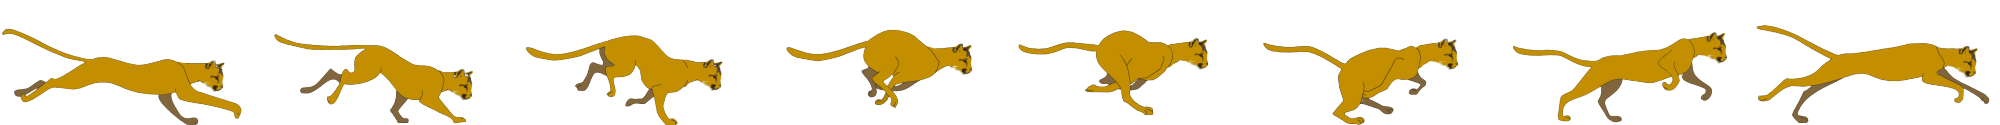
\includegraphics[scale=0.2]{img/cat2.png}
\caption{Kat sprite sheet \cite{catsprite}}
\label{fig:cat}
\end{figure}

\begin{figure}[H]
\centering
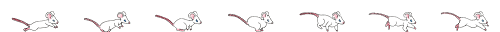
\includegraphics[scale=0.8]{img/mouse2_trans.png}
\caption{Muis sprite sheet \cite{mousesprite}}
\label{fig:mouse}
\end{figure}


\newpage
\subsection{Delaunay}

Voor de animatie wordt gebruik gemaakt van de reeds geschreven delaunay triangulatie. Deze zal het pad vormen waarover de kat of muis zal lopen. Wanneer het dier zich dicht genoeg bij het endPoint bevindt zal deze de firstPoint worden en zullen de buren ervan opgevraagd worden. Er zal willeukeurig een punt worden gekozen als nieuw endPoint. Dit punt kan niet het firstPoint van de vorige beweging zijn. Dit wil zeggen dat de animatie nooit terug op zijn stappen komt. Enkel als de triangulatie een rechte lijn vormt zal de sprite op en neer lopen. 

\subsection{Server/Client side}

De server zal simpelweg de basis info doorgeven aan de client, zelf de berekeningen maken voor de volgende posities en de triangulatie bijhouden. De client krijgt enkel een dictionnary met de x,y positie, de hoek, de frame en een boolean voor spiegeling mee en heeft geen weet van de triangulatie.

\begin{figure}[H]
\centering
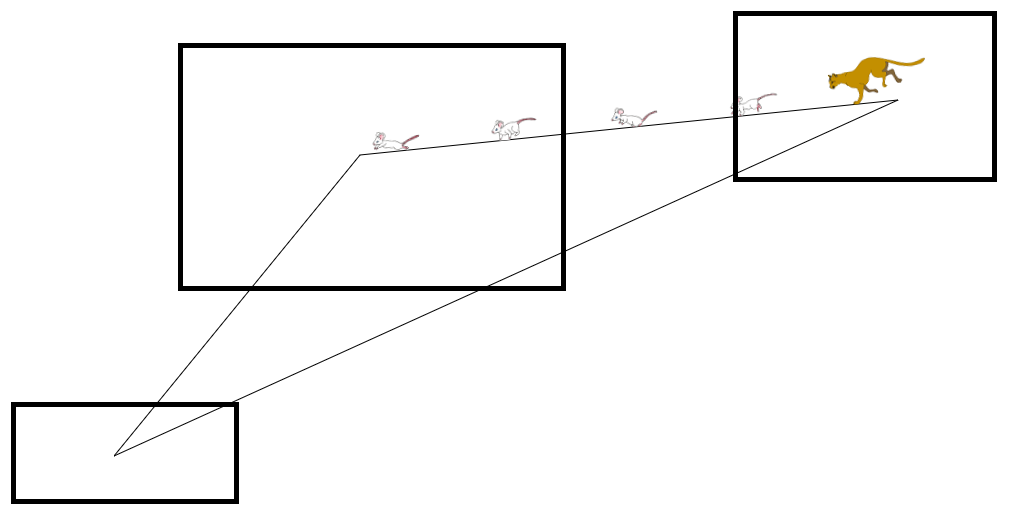
\includegraphics[scale=0.5]{img/schermen.png}
\caption{Theoretische animatie met verschillende schermen}
\label{fig:schermen}
\end{figure}

